\documentclass{beamer}



\usepackage[latin1]{inputenc}
\usepackage[pdftex]{graphicx}
\usepackage{pgf}

\usepackage{pstricks} 
\usepackage{pstricks-add} 
\usepackage{pst-plot} 
\usepackage{pst-text,pst-node,pst-tree} 

\hypersetup{pdfstartview={FitH}}

\setbeamertemplate{navigation symbols}{}
\usetheme{Boadilla}
\title[Point-Based Color Bleeding With Volumes]{PCBEX:\\Point-Based Color Bleeding With Volumes\\Thesis Defense}
\author{Christopher James Gibson}
\institute{California Polytechnic University}
\date{June 9, 2011}

\setcounter{tocdepth}{1}

\begin{document}

\AtBeginSection[]
{
  \begin{frame}<beamer>
    \frametitle{Outline}
    \tableofcontents[currentsection,currentsubsection]
  \end{frame}
}




%%----------------------------------------------------------------------  TITLE
\begin{frame}

    \titlepage

\end{frame}




%%-------------------------------------------------------------------  SCHEDULE
\begin{frame}{Schedule}

\tableofcontents

\end{frame}




\section{Introduction}
%%---------------------------------------------------------------  INTRODUCTION
\begin{frame}{Graphics Intro}

    \begin{columns}
        \begin{column}{0.65\textwidth}
            Definition of Graphics\\
            Graphics and Light\\
        \end{column}
        \begin{column}{0.35\textwidth}
            \rput[lt](0,0){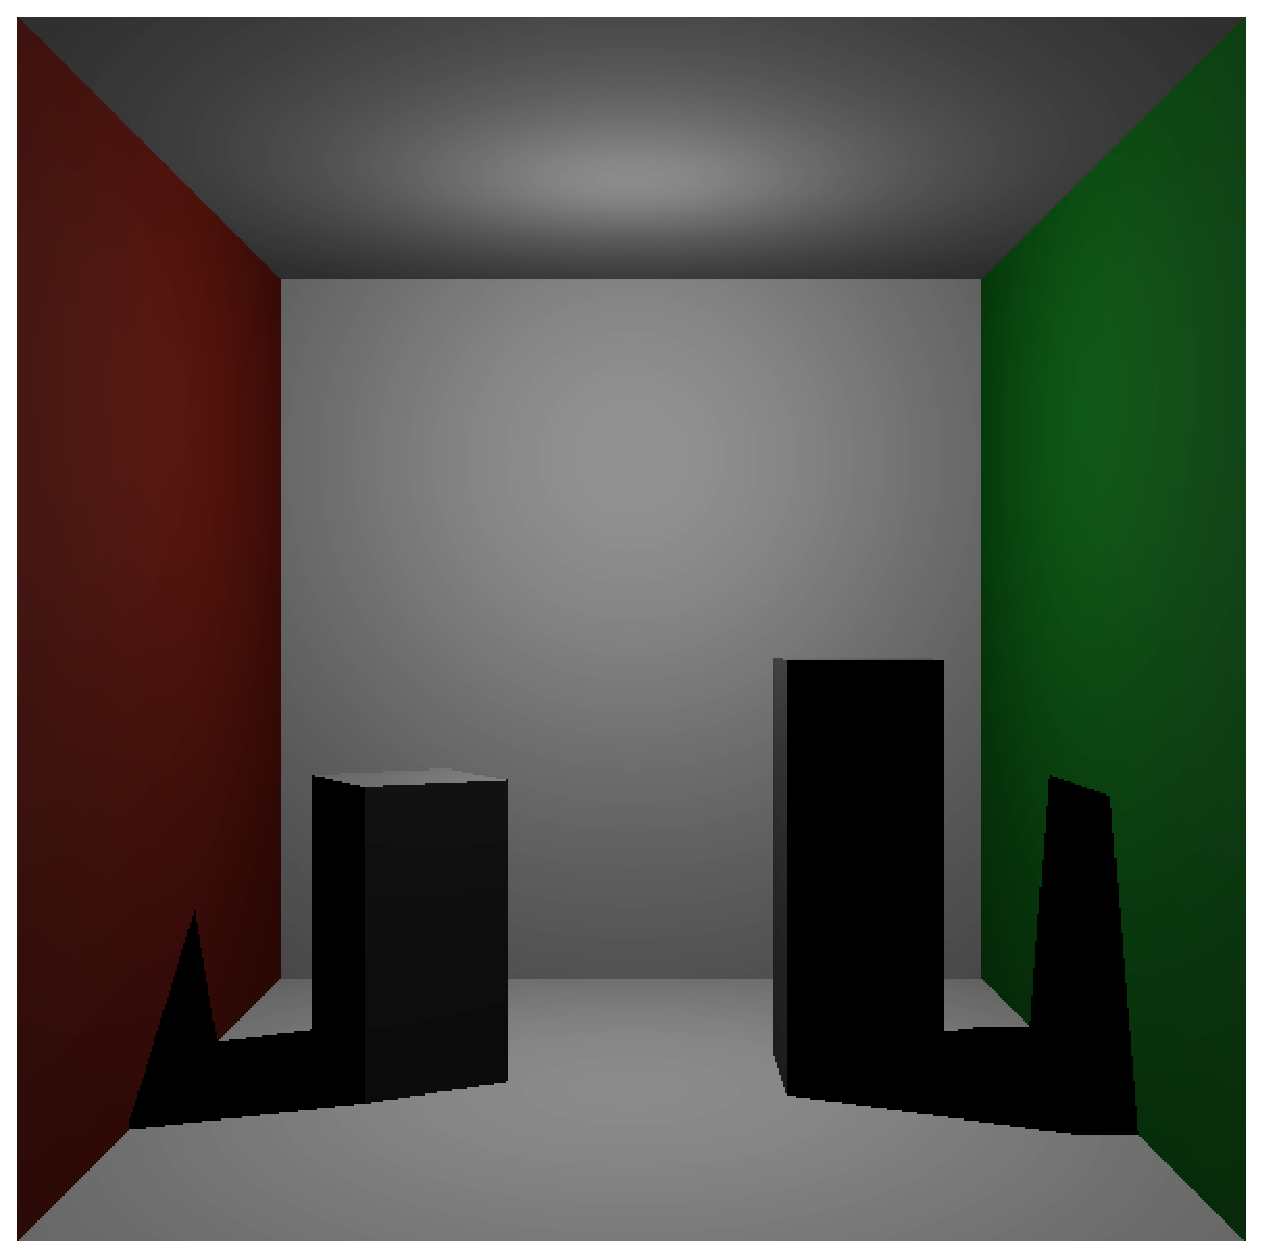
\includegraphics[width=\textwidth]{../img/boxes_noindirect}}
        \end{column}
    \end{columns}

\end{frame}




\subsection{Global Illumination}
%%--------------------------------------------  BACKGROUND: GLOBAL ILLIMUNATION
\begin{frame}{Global Illumination}

    \begin{columns}
        \begin{column}{0.65\textwidth}
            Definition of Graphics\\
            Graphics and Light\\

        \end{column}
        \begin{column}{0.35\textwidth}
            \rput[lb](0,0){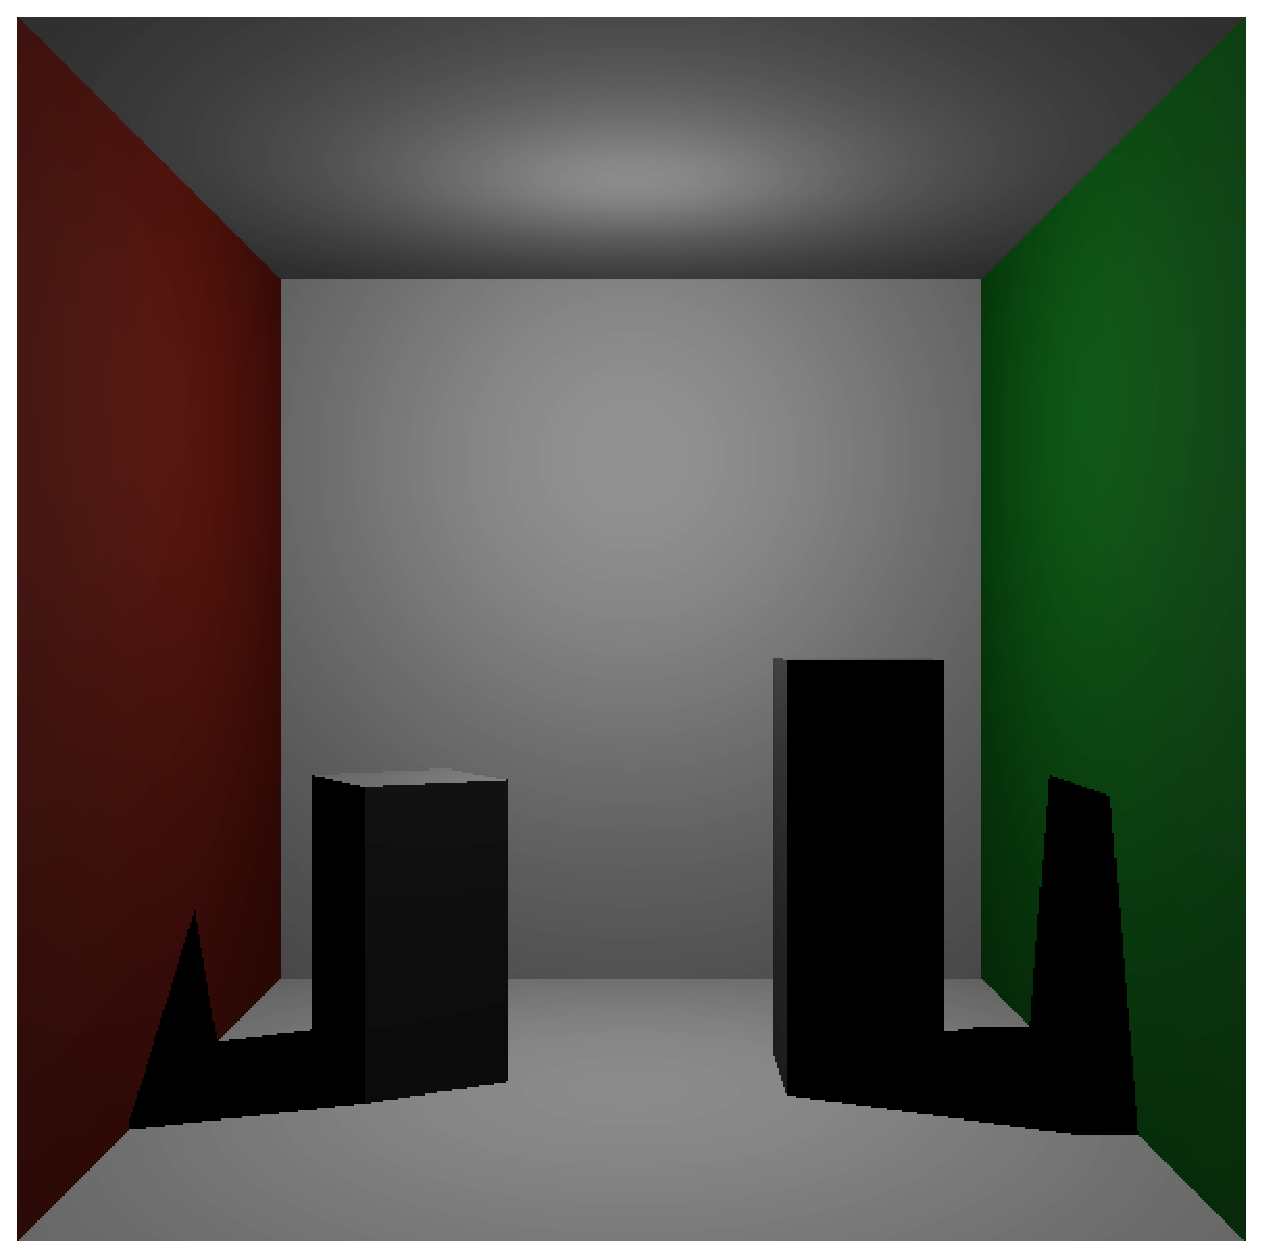
\includegraphics[width=\textwidth]{../img/boxes_noindirect}}
            \rput[lt](0,0){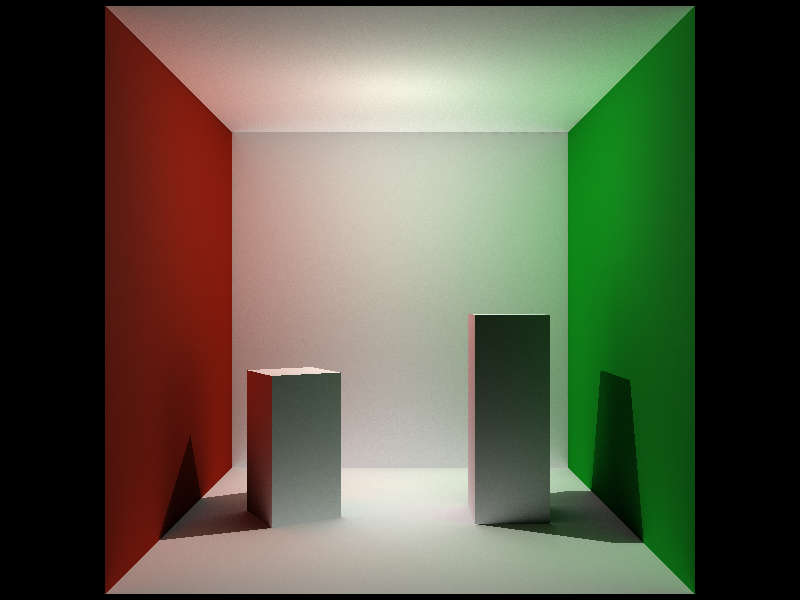
\includegraphics[width=\textwidth]{../img/indirect_box_high}}
        \end{column}
    \end{columns}

\end{frame}




\subsection{Point-Based Color Bleeding}
%%------------------------------------------------  BACKGROUND: VOLUME LIGHTING
\begin{frame}{Point-Based Color Bleeding}

    Oh yea!

\end{frame}




\subsection{Our Contribution}
%%------------------------------------------  RELATED WORK: GLOBAL ILLIMUNATION
\begin{frame}{Our Contribution}

    Oh yea!

\end{frame}




\section{Background}
\subsection{Graphics Background}
%%-----------------------------------------------------------------  BACKGROUND
\subsection{Illumination and Light}
%%---------------------------------------------------  BACKGROUND: ILLIMUNATION
\begin{frame}{Illumination and Light}

    Radiance\\
    BRDF\\
    BSRDF

\end{frame}




\subsection{Volume Lighting}
%%---------------------------------------------------  BACKGROUND: ILLIMUNATION
\begin{frame}{Volume Lighting}

    Oh yea?

\end{frame}




%%-----------------------------------------------  BACKGROUND WORK: MONTE CARLO
\begin{frame}{Monte Carlo Integration}

    Oh yea!

\end{frame}




\section{Related Work}
\subsection{Global Illumination}
%%------------------------------------------  RELATED WORK: GLOBAL ILLIMUNATION
\begin{frame}{Related Works: Global Illumination}

    Oh yea!

\end{frame}




%%------------------------------------------  RELATED WORK: GLOBAL ILLIMUNATION
\begin{frame}{Related Works: Global Illumination}

    Oh yea!

\end{frame}




\subsection{Volume Rendering}
%%---------------------------------------------  RELATED WORK: VOLUME RENDERING
\begin{frame}{Related Works: Volume Rendering}

    Oh yea!

\end{frame}




%%---------------------------------------------  RELATED WORK: VOLUME RENDERING
\begin{frame}{Related Works: Volume Rendering}

    Oh yea!

\end{frame}




\section{PCB Extension Algorithm}
\subsection{Point-Based Color Bleeding}
%%--------------------------------------------------------------  PCB EXTENSION
\begin{frame}{Point-Based Color Bleeding}

    Oh yea!

\end{frame}




\subsection{Extension Overview}
%%--------------------------------------------------------------  PCB EXTENSION
\begin{frame}{Point-Based Color Bleeding}

    Oh yea!

\end{frame}




\subsection{Sampling the Scene}
%%--------------------------------------------------------------  PCB EXTENSION
\begin{frame}{Point-Based Color Bleeding}

    Oh yea!

\end{frame}




\subsection{Gathering Light}
%%--------------------------------------------------------------  PCB EXTENSION
\begin{frame}{Gathering Light}

    Oh yea!

\end{frame}




\subsection{Integrating Volume Data}
%%--------------------------------------------------------------  PCB EXTENSION
\begin{frame}{Integrating Volume Data}

    Oh yea!

\end{frame}




\section{Results}
%%--------------------------------------------------------------------  RESULTS
\begin{frame}{Related Works}

    Oh yea!

\end{frame}




\section{Conclusion}
%%-----------------------------------------------------------------  CONCLUSION
\begin{frame}{Related Works}

    Oh yea!

\end{frame}




\section{References}
%%-----------------------------------------------------------------  REFERENCES
\begin{frame}{Related Works}

    Oh yea!

\end{frame}

\end{document}
